\subsection{Instruction Solver}
An instruction is composed of three fields: {\tt opcode}, {\tt operands} and {\tt modifiers}. An operand can be register, constant memory, global memory, shared memory, immediate, or predicate register.
The encoding of operands can be inferred by their names. For instance, the register operand {\tt R5} could be
inferred as $101$ in binary format, immediate $0x9$ is represented as $1001$. Besides, the fixed lengths of these fields allow us to determine their positions and lengths and hence encoding. Encodings of opcode and modifier are mnemonic symbols, therefore, their encoding can not be speculated by names. Modifiers are instruction specific, the same kind of modifier can be different encodings for different instructions. For instance, mask of type-size
modifier for {\tt LD} and {\tt LDG} are at different positions. So we deal with modifier for each instruction separately.

\subsubsection{Operands:Fixed Length Field}
Algorithm~\ref{algo:int_solver} shows pseudo code for immediate typed operand decoding process. 
The basic idea is that match binary encoding of operand in $64$ instruction encoding and find
position until the postion is unique. The input instructions are from disassembly code (i.e., NVIDIA CUBLAS library).
First, we randomly pick up an instruction that has the field we want to probe, and represent the field in binary by its name. Second, we match the operand binary in $64$-bit instruction encoding, and find possible positions. Third, we intersect current candidates with previous ones, if the number of candidates is $1$, we find the position. Otherwise, we set the current candidate to the previous one and randomly pick next instruction to repeat the procedure.
Other operand type such as register operand can be use similar routine by matching the corresponding operand binary.

\begin{algorithm}
      \caption{Immediate Solver}
      \label{algo:int_solver}
  \begin{algorithmic}[1]
	  \State \textbf{input:} instMap
      \State \textbf{output:} pos, length
      \State currPos=\{\}
      \State prePos=\{0,1,2,...63\}
      \While {length(currpos) != 1}
      \State inst=instMap[random()]
      \If {inst.src1type == immediate}
      \State instEncode=inst->encode64bit
      \State immBin = completement(imm)
      \State pos = 0
      \While {pos+length(immBin) < 64}
      \If {strcmp(immBin,instEncode+pos,length(immBin)}
      \State pushback(currPos, pos)
      \EndIf
      \EndWhile
      \State currPos = intersect (curpos, prepos)
      \State prePos = currPos
      \State currPos=\{\}
      \EndIf
      \EndWhile
      \State return prePos[0]
  \end{algorithmic}
\end{algorithm}

Once operand position is found, we need to probe or veritify the length of operand encoding. Some are easy to be
deduced, for example, each thread can use at most $256=2^{8}$ registers, we could predict the length of register operand mask to be $8$.
However, other operand types like immediate $0x48$ or subscript of constant memory $C[0x2][0x05]$, are more complicated to predicate. Our solution is to set the bit from the position bit by bit to check whether the operand value is grown as we expected. For instance, by using Algorithm~\ref{algo:int_solver}, we find out that the immediate operand position of {\tt IADD RX, RY, 0ximm}(RX, RY is arbitrary register operand, 0ximm is immediate operand) is at bit $23$ as shown in Figure~\ref{fig:imm}. As specified in~\cite{cuda2015programming}, NVIDIA GPU use little-endian representation, then we set bit higher than $23$ to $1$ bit by bit, and observe the the disassembled code. Immediate value increases continuely until reaches value {\tt 0x7ffff}, which means that $41\sim23$ is for integer immediate. Even we set bit $42$ to $1$, no {\tt fffff} immediate is got. 

\begin{figure}[htbp]
\begin{center}
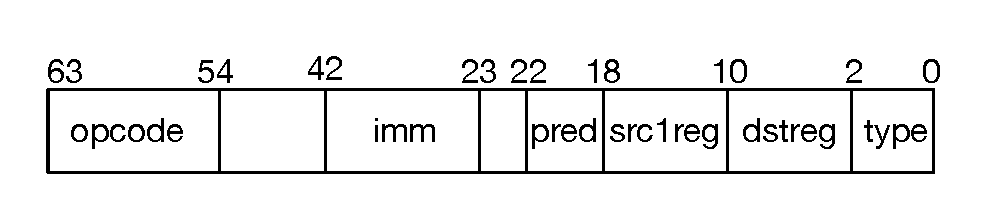
\includegraphics[scale=0.5]{imm}
    \caption{Immediate position at IADD instruction}
\label{fig:imm}
\end{center}
\end{figure}

\subsubsection{Opcode}
Opcodes does not show their encoding literally. One possible way is to write instruction {\tt PTX} code with flags
combinations based on syntax on NVIDIA PTX manual, and generate encoding by using NVDIA toolchain.
Then, opcode can be got by stripping out operand mask, and flags can be found by stripping out opcode and operand mask. However, the uncompleteness of NVIDIA document hinder us to find out all the opcodes and instruction modifiers. Another feasible way is to emulate all of possible binary combinations after striping out operand mask.
Normally, each instruction have $3$ register operand, and one $4-bit$ predicate register, we have $64-8*3-4=36$ bits left to probe.
In fact, we can further prune the search space by recognizing possible position by algorithm~\ref{algo:opcode}. By randomly probing bit by bit, we find that the top $10$ bits and lower $2$ bits represent opcode and other bits represent flags. Thus, we only enumerate these opcode bits which generate a acceptable search space. Finally, we find the minimal opcode without any flags. 


\begin{algorithm}
      \caption{Opcode Solver}\label{algo:opcode}
  \begin{algorithmic}[1]
      \State for each instruction in PTX generated database
      \For {i=0; i < num\_inst; i++}
      \For {j=0; j < 64; j ++}
      \If {isoperand(encode[i][j] == 0) and encode[i][j]== 0}
      \State newcode = encode[i][j].setbit(j, 1)
      \State newinst=nvdisasm(newcode)
      \If {sameop(newinst,oldinst) == 0 and isvalid(newinst) }
      \State pushback(j)
      \EndIf
      \EndIf
      \EndFor
      \EndFor
  \end{algorithmic}
\end{algorithm}

\subsubsection{Modifier: Instruction Specific}

Modifier defines a specific behavior for some instruction. For example,
{\tt LD} instruction has type-size modifiers, such as .u8, .s8, .u16, .32, .64 and .128. {\tt LD} also has cache operation modifier, such as .ca(cache at all level) and .cg(cache at global level). Modifiers (also called flags) are much more complicated because its position spans accross the reminding bits and one instruction may have more than one kinds of modifiers. By excluding both opcode and operand mask, there remain around $24$ bits. We observe that the default value for modifier is $0$. That is, modifier works when at least one bit is set. We can find possible positions of modifiers 
by greedily set the remaining bits one by one, the time complexity is $O(2^{10})$ instead of $O(2^{24})$. The number of bit is typically less
than $10$. After finding the candidates, we enumerate these bits, and group each kind.


